%-----------------------------------------------------------------------------------------------------------------------------------------------%
%	The MIT License (MIT)
%
%	Copyright (c) 2015 Jan Küster
%
%	Permission is hereby granted, free of charge, to any person obtaining a copy
%	of this software and associated documentation files (the "Software"), to deal
%	in the Software without restriction, including without limitation the rights
%	to use, copy, modify, merge, publish, distribute, sublicense, and/or sell
%	copies of the Software, and to permit persons to whom the Software is
%	furnished to do so, subject to the following conditions:
%	
%	THE SOFTWARE IS PROVIDED "AS IS", WITHOUT WARRANTY OF ANY KIND, EXPRESS OR
%	IMPLIED, INCLUDING BUT NOT LIMITED TO THE WARRANTIES OF MERCHANTABILITY,
%	FITNESS FOR A PARTICULAR PURPOSE AND NONINFRINGEMENT. IN NO EVENT SHALL THE
%	AUTHORS OR COPYRIGHT HOLDERS BE LIABLE FOR ANY CLAIM, DAMAGES OR OTHER
%	LIABILITY, WHETHER IN AN ACTION OF CONTRACT, TORT OR OTHERWISE, ARISING FROM,
%	OUT OF OR IN CONNECTION WITH THE SOFTWARE OR THE USE OR OTHER DEALINGS IN
%	THE SOFTWARE.
%	
%
%-----------------------------------------------------------------------------------------------------------------------------------------------%


%============================================================================%
%
%	DOCUMENT DEFINITION
%
%============================================================================%

%we use article class because we want to fully customize the page and dont use a cv template
\documentclass[10pt,A4]{article}	


%----------------------------------------------------------------------------------------
%	ENCODING
%----------------------------------------------------------------------------------------

%we use utf8 since we want to build from any machine
\usepackage[utf8]{inputenc}		

%----------------------------------------------------------------------------------------
%	LOGIC
%----------------------------------------------------------------------------------------

% provides \isempty test
\usepackage{xifthen}

%----------------------------------------------------------------------------------------
%	FONT
%----------------------------------------------------------------------------------------

% some tex-live fonts - choose your own

%\usepackage[defaultsans]{droidsans}
%\usepackage[default]{comfortaa}
%\usepackage{cmbright}
\usepackage[default]{raleway}
%\usepackage{fetamont}
%\usepackage[default]{gillius}
%\usepackage[light,math]{iwona}
%\usepackage[thin]{roboto} 

% set font default
\renewcommand*\familydefault{\sfdefault} 	
\usepackage[T1]{fontenc}

% more font size definitions
\usepackage{moresize}		


%----------------------------------------------------------------------------------------
%	PAGE LAYOUT  DEFINITIONS
%----------------------------------------------------------------------------------------

%debug page outer frames
%\usepackage{showframe}			


%define page styles using geometry
\usepackage[a4paper]{geometry}		

% for example, change the margins to 2 inches all round
\geometry{top=.5cm, bottom=-.6cm, left=-0.1cm, right=0cm} 	

%use customized header
\usepackage{fancyhdr}				
\pagestyle{fancy}

%less space between header and content
\setlength{\headheight}{-5pt}		


%customize entries left, center and right
\lhead{}
\chead{}
\rhead{}

\newcommand{\padding}{1cm}
\newcommand{\innerwidth}{\linewidth-\padding-\padding}

%indentation is zero
\setlength{\parindent}{0mm}

%----------------------------------------------------------------------------------------
%	TABLE /ARRAY DEFINITIONS
%---------------------------------------------------------------------------------------- 

%for layouting tables
\usepackage{multicol}			
\usepackage{multirow}

%extended aligning of tabular cells
\usepackage{array}

\newcolumntype{x}[1]{%
>{\raggedleft\hspace{0pt}}p{#1}}%


%----------------------------------------------------------------------------------------
%	GRAPHICS DEFINITIONS
%---------------------------------------------------------------------------------------- 

%for header image
\usepackage{graphicx}

%for floating figures
\usepackage{wrapfig}
\usepackage{float}
%\floatstyle{boxed} 
%\restylefloat{figure}

%for drawing graphics		
\usepackage{tikz}				
\usetikzlibrary{shapes, backgrounds,mindmap, trees}


%----------------------------------------------------------------------------------------
%	Color DEFINITIONS
%---------------------------------------------------------------------------------------- 
\usepackage{transparent}
\usepackage{color}

%accent color
\definecolor{sectcol}{RGB}{255,150,0}

%dark background color
\definecolor{bgcol}{RGB}{110,110,110}

%light background / accent color
\definecolor{softcol}{RGB}{225,225,225}

% light bg
\definecolor{light}{RGB}{200, 200, 200}

%============================================================================%
%
%
%	DEFINITIONS
%
%
%============================================================================%

%----------------------------------------------------------------------------------------
% 	HEADER
%----------------------------------------------------------------------------------------

% remove top header line
\renewcommand{\headrulewidth}{0pt} 

%remove botttom header line
\renewcommand{\footrulewidth}{0pt}	  	

%remove pagenum
\renewcommand{\thepage}{}	

%remove section num		
\renewcommand{\thesection}{}			

%----------------------------------------------------------------------------------------
% 	ARROW GRAPHICS in Tikz
%----------------------------------------------------------------------------------------

% a six pointed arrow poiting to the left
\newcommand{\tzlarrow}{(0,0) -- (0.2,0) -- (0.3,0.2) -- (0.2,0.4) -- (0,0.4) -- (0.1,0.2) -- cycle;}	

% include the left arrow into a tikz picture
% param1: fill color
%
\newcommand{\larrow}[1]
{\begin{tikzpicture}[scale=0.58]
	 \filldraw[fill=#1!100,draw=#1!100!black]  \tzlarrow
 \end{tikzpicture}
}

% a six pointed arrow poiting to the right
\newcommand{\tzrarrow}{ (0,0.2) -- (0.1,0) -- (0.3,0) -- (0.2,0.2) -- (0.3,0.4) -- (0.1,0.4) -- cycle;}

% include the right arrow into a tikz picture
% param1: fill color
%
\newcommand{\rarrow}[1]
{\begin{tikzpicture}[scale=0.7]
	 \filldraw[fill=#1!100,draw=#1!100!black]  \tzrarrow
 \end{tikzpicture}
}



%----------------------------------------------------------------------------------------
%	custom sections
%----------------------------------------------------------------------------------------

% create a coloured box with arrow and title as cv section headline
% param 1: section title
%
\newcommand{\cvsection}[1]
{
\colorbox{sectcol}{\mystrut \makebox[1\linewidth][l]{
\larrow{bgcol} \hspace{-8pt} \larrow{bgcol} \hspace{-8pt} \larrow{bgcol} \textcolor{white}{\textbf{#1}}\hspace{4pt}
}}\\
}

%create a coloured arrow with title as cv meta section section
% param 1: meta section title
%
\newcommand{\metasection}[2]
{
\begin{tabular*}{1\textwidth}{p{2cm} p{11cm}}
\larrow{bgcol}	\normalsize{\textcolor{sectcol}{#1}}&#2\\[8pt]
\end{tabular*}
}

%----------------------------------------------------------------------------------------
%	 CV EVENT
%----------------------------------------------------------------------------------------

% creates a stretched box as cv entry headline followed by two paragraphs about 
% the work you did
% param 1:	event time i.e. 2014 or 2011-2014 etc.
% param 2:	event name (what did you do?)
% param 3:	institution (where did you work / study)
% param 4:	what was your position
% param 5:	some words about your contributions
%
\newcommand{\cvevent}[5]
{
\vspace{8pt}
	\begin{tabular*}{0.6\linewidth}{ p{12cm} x{3cm}}
\textbf{#2} \textcolor{bgcol}{(#3)}&\textcolor{bgcol}{#1}\\[4pt]
	\end{tabular*}
\vspace{-12pt}
\textcolor{softcol}{\hrule}
\vspace{6pt}
	\begin{tabular*}{1\textwidth}{l}
		 \larrow{sectcol}  #4\\[4.5pt]
		 \larrow{sectcol}  #5\\[6pt]
	\end{tabular*}

}

% creates a stretched box as 
\newcommand{\cveventmeta}[2]
{
	\mbox{\mystrut \hspace{87pt}\textit{#1}}\\
	#2
}

%----------------------------------------------------------------------------------------
% CUSTOM STRUT FOR EMPTY BOXES
%----------------------------------------- -----------------------------------------------
\newcommand{\mystrut}{\rule[-.3\baselineskip]{0pt}{\baselineskip}}

%----------------------------------------------------------------------------------------
% CUSTOM LOREM IPSUM
%----------------------------------------------------------------------------------------
\newcommand{\lorem}
{Lorem ipsum dolor sit amet, consectetur adipiscing elit. Donec a diam lectus.}



%============================================================================%
%
%
%
%	DOCUMENT CONTENT
%
%
%
%============================================================================%
\begin{document}

%use our custom fancy header definitions
\pagestyle{fancy}	

%----------------------------------------------------------------------------------------
% HEADLINE / BASIC INFORMATION
%----------------------------------------------------------------------------------------
\fcolorbox{bgcol}{bgcol}{
\begin{minipage}[c][0.1\textheight][t]{\linewidth}
\begin{center}
	\vspace{14pt}
	\textcolor{light}{\small{Consultant and Software Engineer $\cdot$  Bremen, Germany  $\cdot$  info@jankuester.com  $\cdot$ +49 176 313 XXX XX}}\\[4pt]
	\HUGE{\textcolor{white}{\textsc{Jan Küster}} } \textcolor{sectcol}{\rule[-1mm]{1mm}{0.9cm}} \HUGE{\textcolor{white}{\textsc{Resume}} }
\end{center}
\end{minipage}}\\[-4pt]
%----------------------------------------------------------------------------------------
% SUMMARY
%----------------------------------------------------------------------------------------
\fcolorbox{sectcol}{sectcol}{
\begin{minipage}[c][0.04\textheight][t]{\linewidth}
\begin{center}
\parbox[b]{0.75\linewidth}{
	\begin{center}
	\large
	\larrow{bgcol}\larrow{bgcol} \textcolor{white}{I create awesome resume templates in LaTeX for everyone.} \rarrow{bgcol}\rarrow{bgcol}
	\end{center}
}
\end{center}
\end{minipage}}\\[-4pt]
%----------------------------------------------------------------------------------------
% META
%----------------------------------------------------------------------------------------
\fcolorbox{white}{white}{
\begin{minipage}[c][0.16\textheight][t]{\linewidth}
\vspace{8pt}
\begin{center}
\parbox[c]{\innerwidth}{
	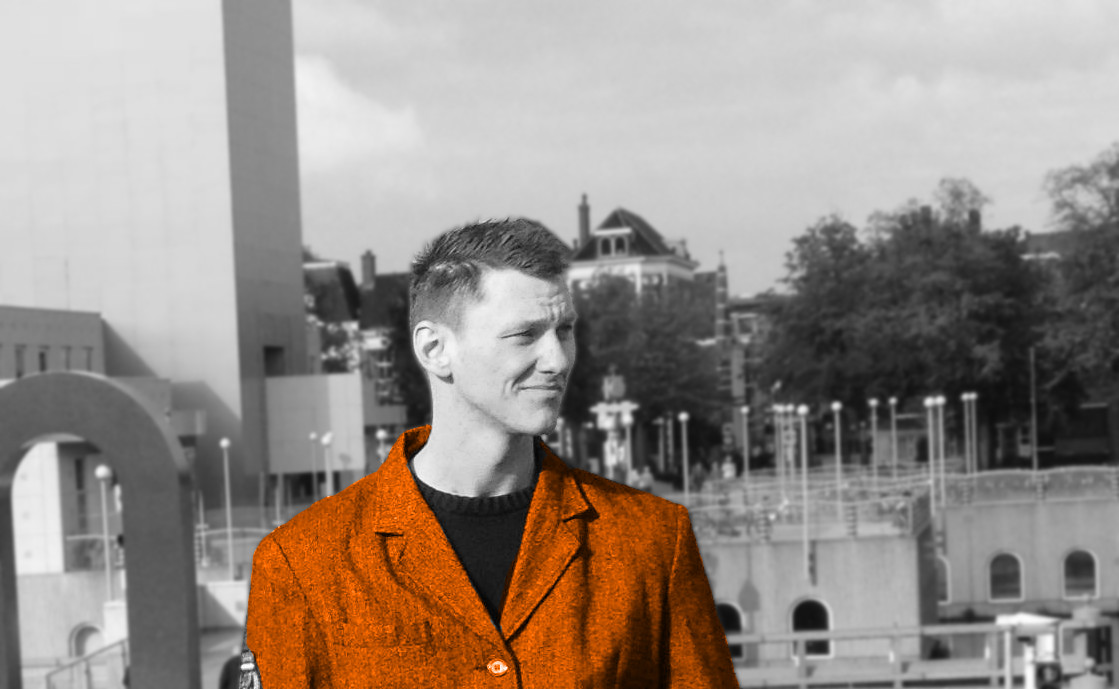
\includegraphics[trim= 320 130 460 210,clip,width=0.2\linewidth]{myfoto.jpg}
	\hspace{8pt}
	\parbox[b]{5cm}{
	\metasection{Status:}{PhD student, M.Sc. Digital Media, Fullstack JS Engineer}
	\metasection{Fields:}{Software Development, Consulting, Education} 
	\metasection{Stack:}{Meteor, Mongo, React, Bootstrap, Fontawesome ,Mocha}
	\metasection{Tools:}{Git, Sourcetree, Travis, Webstorm, Terminal}
	\metasection{Activities:}{Global Game Jam, Sound Engineering, Blender, Martial Arts}
	}
}
\end{center}
\end{minipage}}\\[-4pt]
%----------------------------------------------------------------------------------------
% EXPERIENCE
%----------------------------------------------------------------------------------------
\fcolorbox{light}{light}{
\begin{minipage}[c][0.4\textheight][t]{\linewidth}
\vspace{8pt}
\hspace{20pt}
\parbox[c]{0.75\linewidth}{
%---------------------------------------------------------------------------------------
%	EXPERIENCE
%----------------------------------------------------------------------------------------
%\cvsection{Experience}

%
\cvevent{2016 - now}{Fullstack Javascript Engineer}{University of Bremen}{Invent a realtime classroom management using Meteor and React}{Design software architecture and leading development}

%\textcolor{softcol}{\hrule}

%
\cvevent{2014 - 2016}{IT Consultant for IBM XPages and Notes Domino}{We4IT GmbH Bremen}{Realize projects in XPages and We4IT Aveedo, monitor project status, conduct reports}{Integrated Camunda BPMN engine and BPMN.IO modeler in We4IT Aveedo}


%\textcolor{softcol}{\hrule}

%
\cvevent{2012 - 2014}{Scientific Employee / Software Development}{University of Bremen}{Invented a flexible assessment framework, targeting industrial trainees}{Supervised software development lifecycle, Recruited team members}

%\textcolor{softcol}{\hrule}

%
\cvevent{Nov. 2011}{Project Management Simulation Training}{Getoq Consulting}{Performed a two-day project simulation from management perspective}{Topics included customer contracts, change management, controlling, operational tasks}

%\textcolor{softcol}{\hrule}


%
\cvevent{2010 - 2011}{Student Assistant / Programmer}{otulea.uni-bremen.de}{Realized an online diagnosis platform for workforce literacy development (Flex)}{Modeled software design, implemented various prototypes, conducted usability tests}

}
\hspace{18pt}
\textcolor{sectcol}{\rule[-3.2cm]{2pt}{7cm}}
\hspace{12pt}
\rotatebox[origin=c]{270}{\HUGE \textsc{Experience}}
\end{minipage}}\\[-4pt]


%---------------------------------------------------------------------------------------
%	QR CODE (optional)
%----------------------------------------------------------------------------------------
%\vspace{-136pt}
%\hspace{0.75\linewidth}
%
\includegraphics[width=103pt]{qrcode}
%\normalsize
%\vspace{88pt}
%---------------------------------------------------------------------------------------
%	SUMMARAY (optional)
%----------------------------------------------------------------------------------------

%\cvsection{Summary}\\
%Digital media graduate with four years project experience in the field of technology based assessment. Specialized in development of test-scenario engines and innovative, rich media item formats. Master studies focused on teams from different disciplines and cultural backgrounds on solutions for complex problems.  Prior knowledge has been collected in he field of usability / accessibility during bachelor studies.\\

%============================================================================%
%
%	CV SECTIONS AND EVENTS (MAIN CONTENT)
%
%============================================================================%



%---------------------------------------------------------------------------------------
%	EDUCATION SECTION
%--------------------------------------------------------------------------------------
%\cvsection{Education}

%\cvevent{2015 / 07}{Graduated as M.Sc. Digital Media}{University of Bremen}{Master Thesis: Semi Automated Scoring in Technology Based Assessment}{Developed and evaluated an algorithm for semi automated scoring of spreadsheet data}

%\textcolor{softcol}{\hrule}

%
%\cvevent{2012 - 2013}{Master Project - PrIMA}{University of Bremen}{Co-Invented a touch table application for medical support, co-developed software (Java) }{Formed a scrum team, mainted project dev server (Debian), surveyed target audience}

%\textcolor{softcol}{\hrule}

%
%\cvevent{2012 - 2015}{Master Studies Digital Media}{University of Bremen}{Inter-cultural classes in English, covering special topics in computer science and design}{Professionalized in research methods, software development and e-assessment}

%\textcolor{softcol}{\hrule}

%
%\cvevent{2009 - 2010}{Semester Abroad}{University of Melbourne}{Mastered six months of study and trans-cultural experience in Melbourne, Australia}{Finished machine programming, information visualization, professional essay writing}


%-------------------------------------------------------------------------------------------------
%	ARTIFICIAL FOOTER (fancy footer cannot exceed linewidth) 
%--------------------------------------------------------------------------------------------------

\null
\vspace*{\fill}
\hspace{-0.25\linewidth}\colorbox{bgcol}{\makebox[1.5\linewidth][c]{\mystrut \small \textcolor{white}{www.jankuester.com} $\cdot$ \textcolor{white}{github.com/jankapunkt}}}




%============================================================================%
%
%
%
%	DOCUMENT END
%
%
%
%============================================================================%
\end{document}
